\chapter{Related Work}
In this section, recent work on target search methods, multi-robot task allocation, and routing constraints is reviewed.

\section{Target Search}
Searching for targets in an environment is a sequential decision-making problem. Therefore, search methods based on the type of decision-making algorithm, such as submodular approaches, the frontier-based search, the next-best-view search, the probabilistic search, and Partially Observable Markov Decision Processes (POMDP), can be adopted to generate the search strategies.

The submodular method formulates the target search problem as submodular maximization under a resource constraint.
Singh et al. \cite{singh2007efficient} introduce an efficient path planning algorithm (eMIP), which coordinates multiple robots to obtain highly informative paths subject to the robot's path cost.
The eMIP finds solutions that achieves at least $\frac{1-1/e}{1+\log_2 N}$, where $N$ is the number of robots.
However, the performance deteriorates when more robots are involved.
Li et al. \cite{li2024mrsis} propose a Multi-Robot Search with an Intersection System (MRSIS) algorithm.
The objective is to generate a set of robot trajectories that maximize a coverage function and balance robot workloads under clustering and routing cost constraints.
The clustering and routing constraints are formulated as an intersection system.

The frontier-based search method utilizes the frontier between the explored and unexplored space to expand existing knowledge.
Zhou et al. \cite{zhou2021fuel} propose a hierarchical framework, Fast UAV ExpLoration (FUEL), that supports UAV exploration in complex unknown environments. It improves the exploration efficiency using the incremental frontier information structure.
The work is extended to decentralized multi-UAV\cite{zhou2023racer}.
Instead of allocating frontiers and viewpoints to the UAVs, the task assignment is based on an online hierarchical decomposition to ensure that all UAVs simultaneously explore distinct regions.

The next-best-view (NBV) planning determines the next viewpoint that provides the most valuable information to improve search efficiency.
Mittal et al. \cite{mittal2019vision} adopt NBV planner for exploration and propose a novel landing site detection algorithm that computes costmaps based on several hazard factors (e.g., terrain flatness, steepness, depth accuracy, and energy consumption information).
Lauri et al. \cite{lauri2020multi} propose a submodular utility function for multi-sensor NBV planning under partition matroid constraints. In addition, the utility function coordinates view selection and prevents overlapping views among multiple sensors.

The probabilistic approach is to estimate the target location under sensor and target motion uncertainty.
Robots make decisions based on the probability distribution.
Mohamed et al. \cite{Mohamed2020person} present the person search-orienting problem (PSOP).
It adopts the user activity probability density functions (APDFs) to generate a search plan to maximize the expected target detection with the limited search time. The approach is then extended to multiple robots by generating a team plan to cooperate effectively \cite{Mohamed2022multirobot}.
Sheng et al. \cite{sheng2022pd} propose a probability density factorized (PD-FAC) multi-agent distributional reinforcement learning method that decomposes the PDF of the multi-robot system into a set of individual value distributions. It is guaranteed that the objective function of the overall system’s value distribution can be linearly approximated by the same reliability metric defined over the agent’s individual value distribution.

Formulating robotic search problems as Partially Observable Markov Decision Processes (POMDP) has recently become a popular method.
POMDP considers the search problem where the states of target locations and robot sensors are uncertain.
A sequence of actions is generated by maximizing a reward function.
Zhu et al. \cite{zhu2020approach} propose a Dec-POMDP method to find a target in an environment with obstacles. The approach provides a scalable framework for a large number of UAVs. It enables the UAV swarm to cooperate efficiently by sharing limited observations in the mission.
Many methods constrain the search space in 2D. Zheng et al. \cite{Zheng2021mos3d} present a multi-object search method, 3D Multi-Object Search (3D-MOS), in 3D environments with a frustum-shaped field of view, which can be applied to mobile robots or drones.


\section{Multi-Robot Task Allocation (MRTA)}
The goal of MRTA is to optimize an objective function within a given budget for multiple robots. However, finding an optimal solution is NP-hard \cite{korsah2013comprehensive}.

% matroid
Several research studies have employed submodular maximization with matroid constraints to solve the MRTA problem. This problem involves various challenges, such as the orienteering problem \cite{gunawan2016orienteering}, the intermittent deployment problem \cite{liu2018optimal}, and the capacitated vehicle routing problem \cite{ralphs2003capacitated}.
If the objective function is submodular, greedy algorithms can find solutions with theoretical guarantees\cite{nemhauser1978analysis}.
In the team surviving orienteers (TSO) problem \cite{jorgensen2017matroid},
an independent set of a matroid is selected for maximizing the expected visited nodes at least one robot.
These nodes also ensure that each vehicle reaches its destination with probabilities above a specified threshold.
In environmental monitoring application \cite{liu2019submodular}, the multi-robot task allocation problem and the multi-robot intermittent deployment problem are formulated as submodular maximization with matroid intersection constraints.
In the surveillance task allocation in urban environments \cite{williams2017decentralized}, a decentralized algorithm, which applies auction methods to assign tasks with matroid constraints, is proposed.

% RL
Recent research on multi-robot task allocation has been paying attention to deep reinforcement learning approaches with graph neural network (GNN) \cite{tolstaya2021multi}.
Paul et al. \cite{paull2022learning} propose a Capsule Attention-based Mechanism (CapAM), a graph reinforcement learning architecture that encodes graph information such as robot location, task deadline, and elapsed mission time. The approach can be easily scaled to a large number of tasks.
Tolstaya et al. \cite{tolstaya2021multi} develop a GNN architecture with behavior cloning to solve the coverage problem. Using a sparse representation of the local graph connectivity, the approach can scale to larger maps and teams.
Zhang et al. \cite{zhang2022h2gnn} propose a Hierarchical-Hops Graph Neural Networks (H2GNN), which evaluates the importance of graph nodes at different hops through the multi-head attention mechanism. To improve exploration efficiency, multi-agent reinforcement learning is applied to learn collaborative strategies.


\section{Routing Constraints}
Submodular optimization has been explored with extensive applications in various domains, such as sensor placement \cite{krause2007near}, viral marketing \cite{golovin2011adaptive}, and robotic search problems \cite{Tsai2019spatial}.
To apply submodular optimization in realistic environments, different constraints (e.g., cardinality \cite{nemhauser1978analysis}, additive budget \cite{khuller1999budgeted}, and routing \cite{zhang2016submodular}) must be considered.

Zhang et al. \cite{zhang2016submodular} propose a generalized cost-benefit (GCB) greedy algorithm
to solve two NP-hard problems: monotone submodular maximization and routing path minimization (TSP).
GCB finds solutions that achieves $\frac{1}{2}(1-\frac{1}{e})\widetilde{OPT}$ optimum, where $\widetilde{OPT}$ is the approximated optimum.
However, there is a gap between $\widetilde{OPT}$ and the optimal solution ($OPT$). To improve the theoretical guarantee of GCB, Lin et al. \cite{Lin2023ST} propose Tree-Structured Fourier Supports Set (TS-FSS) algorithms that combine the characteristics of submodularity and sparsity of routing trees to boost the theoretical bound.

Besides, Zhang et al. \cite{zhang2022nonmonontone} investigate the non-monotone submodular maximization with the $k$-independence system routing constraint, where $k$ is loosely upper-bounded by the size of the ground set.
An iterated two-stage algorithm is presented to obatin a $[\frac{1}{4k}, 1+\theta]$-bicriterion approximation solution, where $\theta$ is an error parameter within $(0,1)$.

\begin{figure}
    \centering
    \begin{subfigure}[b]{0.35\textwidth}
        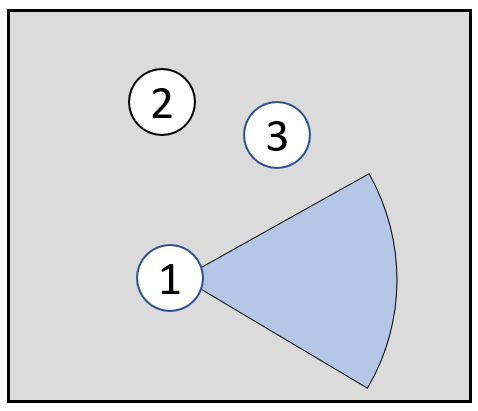
\includegraphics[width=1\textwidth]{cov-1.png}
        \caption{$f(S_A)$}
    \end{subfigure}
    %\hfill
    %\quad
    \begin{subfigure}[b]{0.35\textwidth}
    %\centering
        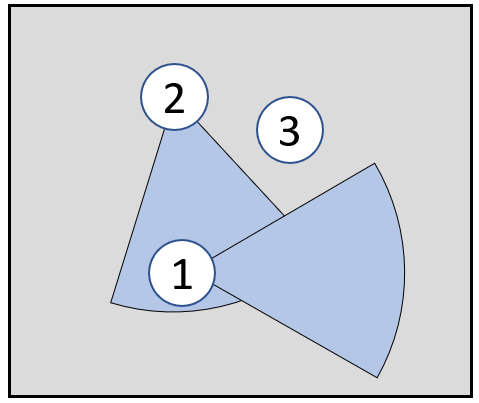
\includegraphics[width=1\textwidth]{cov-2.png}
        \caption{$f(S_B)$}
    \end{subfigure}
    \hfill

    \begin{subfigure}[b]{0.8\textwidth}
    \centering
        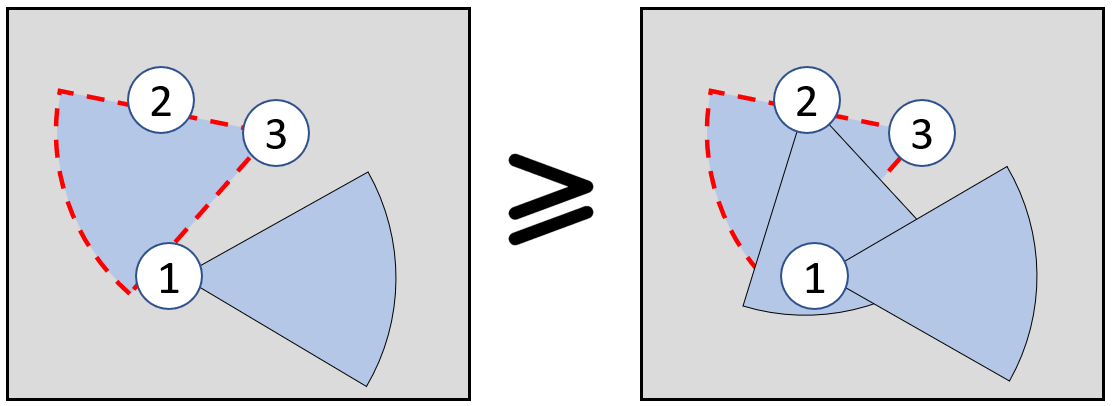
\includegraphics[width=1\textwidth]{cov-12.png}
        \caption{$f(S_A \cup s)-f(S_A) \geq f(S_B \cup s)-f(S_B)$ } \label{fig:AB-cov}
    \end{subfigure}

    \caption{Illustration of submodularity under coverage scenario. The geographical locations of sensors are denoted as decimal numbers, while the blue and gray areas correspond to the covered and uncovered regions, respectively. (a) $f(S_A)$ is the covered area of $S_A$, where $S_A=\{1\}$. (b) $f(S_B)$ is the covered area of $S_B$, where $S_B=\{1,2\}$. (c) The marginal gain of the coverage function $f$ is marked as red dashed lines when $s=\{3\}$ is added to the current set $S_A=\{1\}$ and $S_B=\{1,2\}$.
    }
    \label{submodularity}
\end{figure}


